\documentclass[12pt]{article}
\usepackage{verbatim}
\usepackage[dvips]{epsfig}
\usepackage{color}
\usepackage{url}
\usepackage[colorlinks=true]{hyperref}

\begin{document}

\section*{GENESIS: Documentation}

{\bf Related Documentation:}
% start: userdocs-tag-replace-items related-do-nothing
% end: userdocs-tag-replace-items related-do-nothing

\subsection*{Figure\,5}

\begin{figure}[h]
\centering
   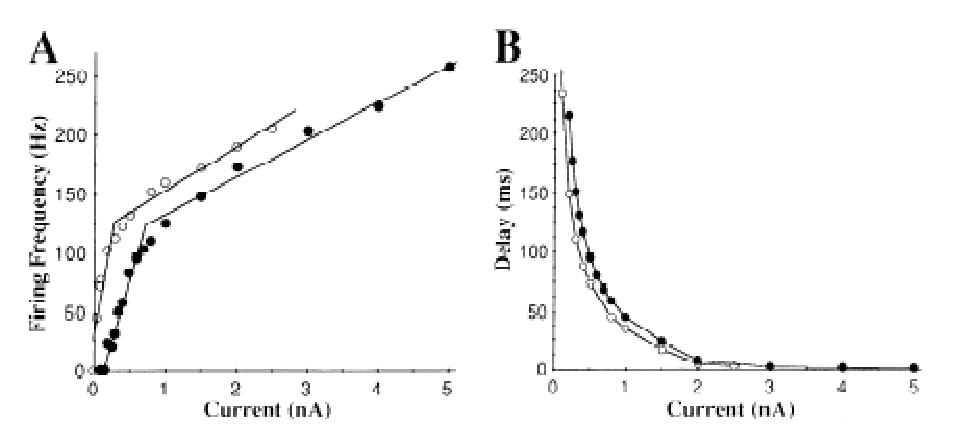
\includegraphics[scale=1]{figures/Fig.1.6.eps}
   \caption{Relation of somatic firing response to the amplitude of injected current in models PM9 ($\circ$) and PM10 ($\bullet$). {\it A}: Firing frequency vs. amplitude of injected current [frequency-current ($f$--$I$) curve]. Frequencies were measured in an interval from 300 to 700\,ms after onset of the current injection, before any clear depolarizing spike bursts in the soma. {\it B}: Delay between onset of current injection and 1st somatic spike vs. amplitude of injected current.}
   \label{fig:DS1.6}
\end{figure}

\bibliographystyle{plain}
\bibliography{../tex/bib/g3-refs.bib}

\end{document}
